% Author: Izaak Neutelings (June 2022)
% Inspiration:
%   "On the dimensionality of spacetime", Max Tegmark
%   https://arxiv.org/abs/gr-qc/9702052
\documentclass[border=3pt,tikz]{standalone}
\usepackage{siunitx}
\usepackage[outline]{contour} % glow around text
\contourlength{1.1pt}
\usetikzlibrary{3d} % for canvas

% STYLE
\tikzset{>=latex}
\tikzstyle{border}=[thick,blue!15!black]

\begin{document}


% DIMENSIONS
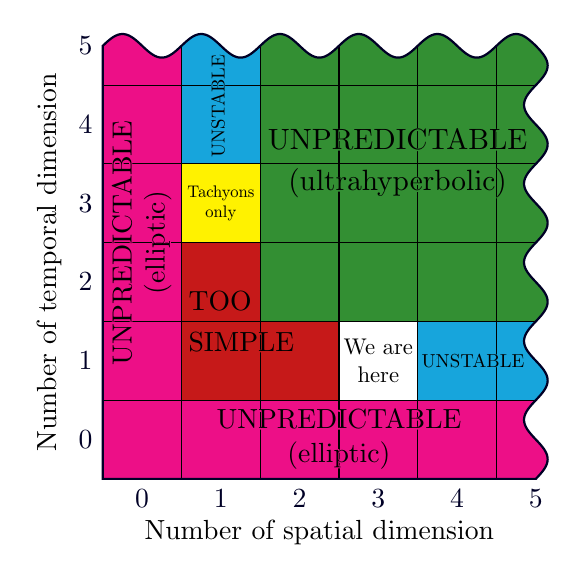
\begin{tikzpicture}[scale=1]
  \def\A{0.15}   % amplitude of sine wave cut off
  \def\xmax{5.5} % maximum dimension
  \def\sinecut{  % path of sine wave cutoff
    (\xmax,0) -| (0,\xmax) -- 
    plot (\x,{\xmax+\A*sin(deg(2*pi*\x)))}) -- (\xmax,\xmax) --
    plot ({\xmax+\A*sin(deg(2*pi*\x)))},\xmax-\x) -- cycle
  }
  
  % CHART
  \colorlet{col-elliptic}{magenta!90!red!95}
  \colorlet{col-unstable}{cyan!90!black}
  \colorlet{col-simplist}{red!75!black!90}
  \colorlet{col-tachyons}{yellow}
  \colorlet{col-unpredic}{green!45!black!80}
  \colorlet{col-werehere}{white}
  \begin{scope}
    \clip[samples=200,domain=0:\xmax] \sinecut;
    \fill[col-elliptic] (0,0) rectangle (6,6); % elliptic
    \fill[col-unstable] (1,1) rectangle++ (6,6); % unstable
    \fill[col-simplist] (1,1) rectangle (3,3); % too simple
    \fill[col-werehere] (3,1) rectangle++ (1,1); % we are here
    \fill[col-tachyons] (1,3) rectangle++ (1,1); % tachyons
    \fill[col-unpredic] (2,2) rectangle (6,6); % unpredictable
    \draw (0,0) grid[step=1] (\xmax,\xmax);
  \end{scope}
  
  % LABELS
  \begin{scope}[every node/.style={align=center}] %font=\bf,font=\ttfamily
    \node at (3,0.5) {
      \contour{col-elliptic}{UNPREDICTABLE}\\
      \contour{col-elliptic}{(elliptic)}
    };
    \node[rotate=90] at (0.5,3) {
      \contour{col-elliptic}{UNPREDICTABLE}\\
      \contour{col-elliptic}{(elliptic)}
    };
    \node[right=-1,align=left] at (1,2) {
      \contour{col-simplist}{TOO}\\[3]
      \contour{col-simplist}{SIMPLE}
    };
    \node[scale=0.6] at (1.5,3.5) {
      \contour{col-tachyons}{Tachyons}\\ %[3]
      \contour{col-tachyons}{only}
    };
    \node[scale=0.6] at (1.5,3.5) {
      \contour{col-tachyons}{Tachyons}\\ %[3]
      \contour{col-tachyons}{only}
    };
    \node[scale=0.82] at (3.5,1.5) {
      \contour{col-werehere}{We are}\\
      \contour{col-werehere}{here}
    };
    \node[right=-1,scale=0.68] at (4,1.5) {
      \contour{col-unstable}{UNSTABLE}
    };
    \node[right=-1,scale=0.68,rotate=90] at (1.5,4) {
      \contour{col-unstable}{UNSTABLE}
    };
    \node[right=-1,scale=1.06] at (2,4) {
      \contour{col-unpredic}{UNPREDICTABLE}\\[2]
      \contour{col-unpredic}{(ultrahyperbolic)}
    };
  \end{scope}
  
  % BORDER
  \draw[border,samples=200,domain=0:\xmax]
    \sinecut;
  
  % AXIS
  \foreach \i [evaluate={\x=\i+0.5;}] in {0,...,5}{
    \node[border,below] at (\x,0) {$\i$};
    \node[border,left] at (0,\x) {$\i$};
  }
  \node[above,rotate=90] at (-0.4,\xmax/2) {Number of temporal dimension};
  \node[below] at (\xmax/2,-0.4) {Number of spatial dimension};
  
\end{tikzpicture}


\end{document}